\section{Species of the MCM and ways to represent them.}\label{sec:drinput}
The master chemical system (as defined in all previous chapters), represents our foremost knowledge of gas phase chemistry within the troposhere. It has been shown that due to its creation protocol (\autoref{fig:protocol}), much of the information about a species structure is encoded within the reaction pathways it can take. This section explores the different methods of representing a species structure, with the aim of providing a machine built algorithm with the greatest amount of information about each species and its functionality. To do this a range of input types will be evaluated against a number of different dimensionality reduction algorithms with the aim of isolating which chemical properties are most `picked up'. 

\subsection{Input generation}
The MCM provides species information in the form of a species `smiles' (\autoref{sec:smiles}) and the IUPAC InChi string \citep{inchi}. Within this chapter we use only the smiles string, which is either manually processed using regular expressions or with the aid of pythons RDKIT package \citep{rdkit}. There are seven different methods for representing the chemsitry, each of which are outlined below. 


\subsection{Manual Categorisation}
Reactions within the MCM are determined by a set of rules (PROTOCOL SECTION). These are designed to mimic the process a chemist my discover new species, and often rely on the bond availability and functionalisation of a species. Since the present functional groups are the benchmark of whether a DR algorithm has sucessfuly separated species structure, it make sense to run a unit test using the known functional groups of a species as the input. 

To genearate the functional groups the regular expressions in \autoref{tab:fngroups} are used\footnote{To see the structure of each functional group type, go to \autoref{appendix:fngroups}.} on the smiles strings (described in \autoref{sec:smiles}) for each species. In extracting the functional groups we are able to plot the likelyness a species with a certain group is likely to have another using a chord diagram - \autoref{fig:covermcm}. Since most species are found to contain a multitude of functional groups, the separation of these into `tidy' clustered groups seems unlikely.      


%
% Except for dissociation, species reactions are often dictated by their functional groups. Species in the MCM are usually represented as functionalised alkanes (A saturated hydrocarbon in the form of $C_nH_{2n+2}$). In removing a hydrogen we form an alkyl chain. This allows for the potential of forming a bond with other atoms. By themselves alkyl chains are mostly un-reactive, however in gaining additional functional groups (functionalisation) their reactivity increases.%



\begin{table}[H]
    \centering
    \begin{tabular}{c|p{5in}}


PAN & \verb! C\\(=O\\)OON\\(=O\\)=O$|^\\[O-{0,1}\\]\\[N\\+{0,1}\\]\\(=O\\)OOC|!\\&\verb! O=N\\(=O\\)OOC\\(=O\\)|C\\(=O\\)OO\\[N\\+{0,1}\\]\\(=O\\)\\[O-{0,1}\\]!\\&\\

Carb. Acid & \verb! [^O](C\\(=O\\)O$|^OC\\(=O\\))!\\&\\

Ester & \verb! [\^O](C\(=O\)O\b|OC\(=O\))C!\\&\\

Ether & \verb! (\([\^O=]+\))*C(\([\^O=]+\))*O(\([\^O=]+\))*C(\([\^O=]+\))*!\\&\\

Per. Acid & \verb! c\\(=O\\)OO$|^OO\\(=O\\)C!\\&\\

% Hydroperoxide & \verb! COO$|C\\(OO|OO\\)C|^OOC!\\&\\

Nitrate & \verb! O(NO2\b|NOO\b|N\(=O\)=O|\[N\+\](?:\[O-\\]|\(=O\)){2})!\\&\\

Aldehyde & \verb! C=O$|^O=C!\\&\\

Ketone & \verb! C\(=O\)C!\\&\\

Alcohol & \verb-CO\\b|(?=^\\b)(?!^\\[)CO.|(?=^\\b)(?!^\\[)OC.|\\(O\\)|C\\)O(\\b|[^O]-\\&\\

Criegee & \verb! \[O-\]\[O\+\]!\\&\\

Alkoxy rad & \verb!\[[\/]{0,1}CH{0,1}\]|\b[\^O]\[O\.{0,1}\]!\\&\\

Peroxyacyl rad & \verb! \\ w\(=O\)O\[O\.{0,1}\]!\\&\\

    \end{tabular}

    \caption{CHECKKKKKKK!!!!!!!!!  A set of regular expressions that may be used to determine the number of occurrences of a functional group within a SMILES string.}
    \label{tab:fngroups}
\end{table}



\begin{figure}[H]
    \centering
    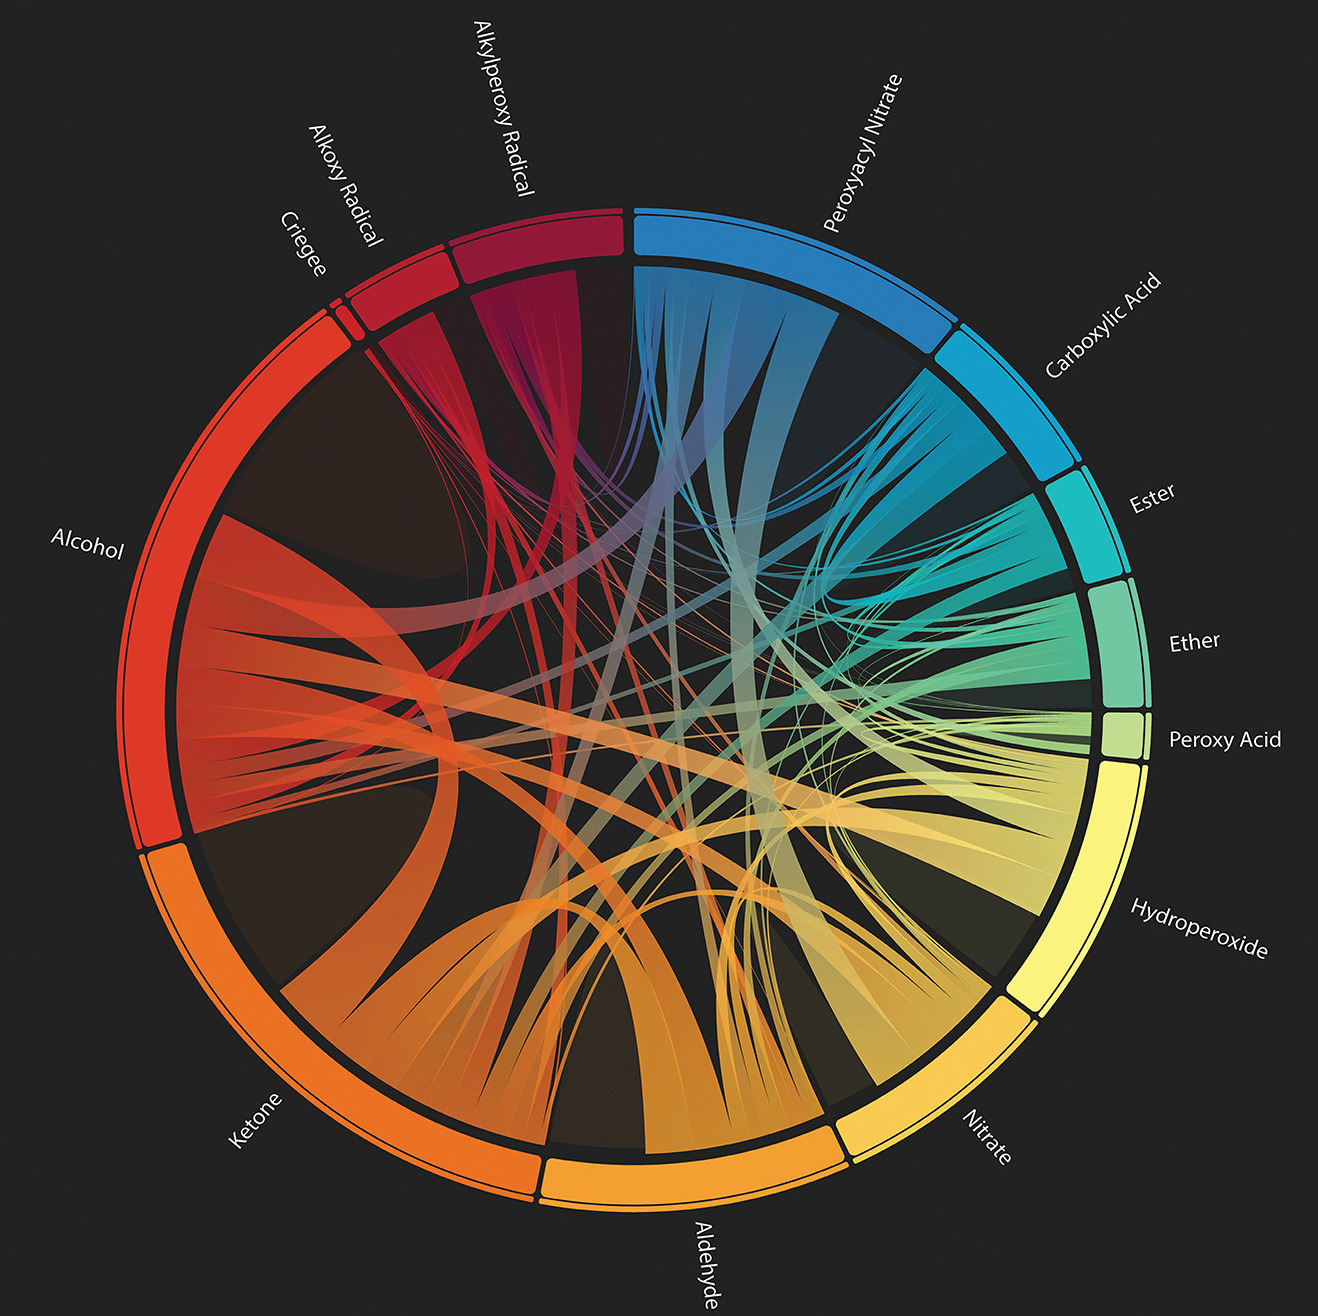
\includegraphics[width=\textwidth]{4fig/coverfig.jpg}
    \caption{\textbf{The multifunctionality of the MCM.} A chord diagram showing the functionalisatoin of a species within the MCM. Arc sizes represent what percentage of all functional groups in the MCM mechanism a group contains. Translucent areas of no outwards links represent species with multiples of a certain functional group, of which Alcohols and Ketones have the most.  
    Source: \citep{cover} }
    \label{fig:covermcm}
\end{figure}



\subsection{Tokenization}
As computer algorithms are unable to understand words, or their meaning, we have to first categorise the data into groups. Tokenisation is the conversion of a string into characters and representing them with a numerical equivalent. In doing so a string of characters can be converted into a numerical vector, allowing for its representation in a latent vector space. 
Within our input selection, we have two sets of inputs we can convert. These are the species names, and their smiles string representation. 



\subsubsection{Species Names}
In \autoref{ch4} it was shown that the dedicated species names for species in the CRI mechanism were often representative of their structural properties. This addage also applies for the MCM, where an intitive naminc convention has been selected. This is is often derrived as part of the construction protocol, where a species names reflects its own, or its precursors structure (which it will have atleast in-part inherited).

Although this is not the most robust method of defining structure, it allows for an easy test of the algorithms, for which the user can quickly compare the human readable output. 

%\begin{table}[H]
%\centering
%\begin{tabular}{lr}
% \textbf{Suffix}&\textbf{Kind}  \\
% \hline &\\
% OH / OL & Alcohol\\
% AL & Aldehyde \\
% ANE & Alkanes\\
% ENE & Alkene\\
% % ATE & ESTER \\
% ER & ETHER\\
% ONE & KETONE
%\end{tabular}\caption{A table of some of the more common suffixes within the MCM.}\label{suffix}
%\end{table}



\subsubsection{SMILES strings}\label{sec:smiles}


 Smiles (`Simplified Molecular-Input Line-Entry System') provide a human-readable representation of molecular structure,
 \citep{smiles}. They provide a linear human-readable representation of the chemical structure within a molecule. This makes it easy for us to visually check the structure of a species without any additional work. In addition their role in generating the molecular fingerprints in \autoref{sec:fingerprints} makes it a useful comparison to make when evaluating methods of structure representation. 

\paragraph*{Construction Methodoly of SMILES strings}
Smiles strings are constructed in three parts. We begin with a species backbone, then add break cycles and branches producing a smiles string. A visual description of this procedure is given below. 

\begin{enumerate}
    \item The smiles string is built by creating the longest possible chain to form a molecule backbone.
    \autoref{fig:st2}

    \item This may within itself contain aromatic rings denoted by the lowercase carbons and a number corresponding to the location of each break cycle. \autoref{fig:st3}

    \item Finally all the functional groups and branches attached to the main backbone are added. These are nested within parenthesis to show that they are not part of the skeletal backbone. \autoref{fig:st4}
\end{enumerate}



\begin{figure}[H]
     \centering
     \begin{subfigure}[b]{0.495\textwidth}
         \centering
         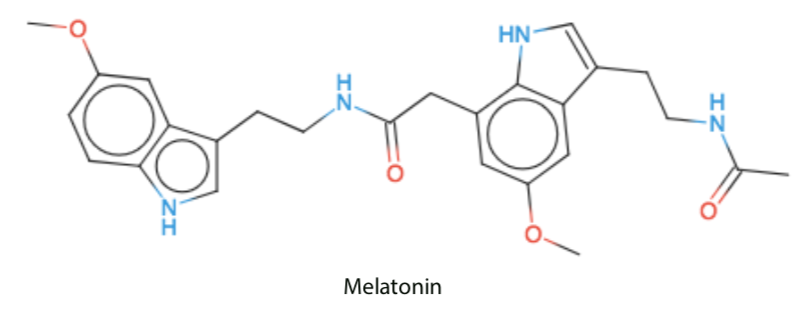
\includegraphics[width=\textwidth]{4fig/sm4.png}
         \caption{Structure of Melatonin}
         \label{fig:st1}
     \end{subfigure}
     \hfill
     \begin{subfigure}[b]{0.495\textwidth}
         \centering
         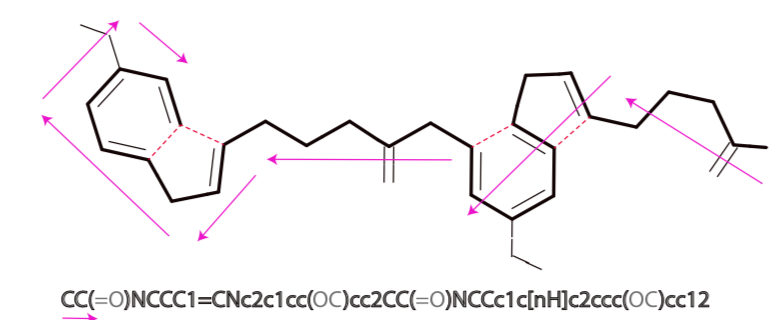
\includegraphics[width=\textwidth]{4fig/sm1.png}
         \caption{Step 1 : Building the C chain backbone.}
         \label{fig:st2}
     \end{subfigure}\\

     \begin{subfigure}[b]{0.495\textwidth}
         \centering
         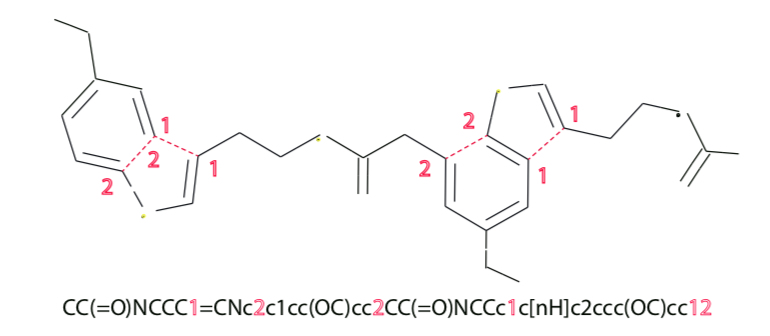
\includegraphics[width=\textwidth]{4fig/sm3.png}
         \caption{Step 2 : Aromatic Rings}
         \label{fig:st3}
     \end{subfigure}
     \hfill
     \begin{subfigure}[b]{0.495\textwidth}
        \centering
            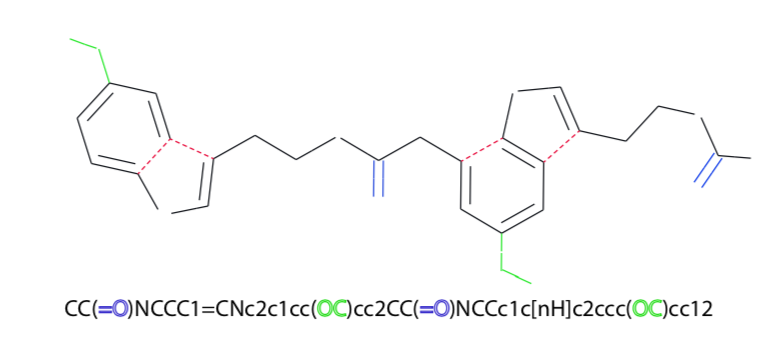
\includegraphics[width=\textwidth]{4fig/sm2.png}
            \caption{Step 3 : Functional Groups }
            \label{fig:st4}
        \end{subfigure}

        \caption{ \textbf{Construction process of a smiles string.} The example compound is Melatonin. Although this does not exist within the atmosphere, it provides a clear example of the smiles string methodology. \autoref{fig:st1} is made using smiles drawer: \citep{smilesdrawer} }
        \label{fig:smiles}
\end{figure}


\subsubsection{Graph Inspired}

\autoref{ch2} - \ref{ch4} have shown the role of graphs in revealing network properties and structure. Graphs in themselves are able to simplify relational data into two/three dimensions for visualisation and algorithmic clustering. Continuing this trend we can represent a species strucuture in the form of a graph (\autoref{sec:specgraph}), as well as converting the structure of a mechanism for dimensionality reduction (\autoref{sec:n2vec})


\paragraph{The species graph}\label{sec:specgraph}

As noted in \citep{mcmgen}, it is possible to represent molecular structure to
a computer using a bond matrix. A bond matrix is the adjacency matrix derived from representing a molecule in the form of a simple graph - where nodes represent atoms and edges the bonds between them. This means that we can take the ball-stick structure of a chemical species \autoref{fig:graphmol}, and convert it into a relation matrix with values corresponding to the number of nodes \autoref{fig:adjmol} This is similar to the concept of z-matrixes, which are often used in chemistry to represent atoms in a molecule in the form of Cartesian coordinates through the use of bonds, and bond angles \citep{zmatrix}.

Since we wish to compare species of differing numbers of atoms, \autoref{table:my_maxoccur}, we create a universal matrix capable of containing any foreseeable bond-atom combination in the form of a subgraph. This produces a $37^2$ element adjacency matrix. The above matrix can now be flattened (separated into rows with each row joined in series to produce a single array of dimension [1,$37^2$]). This produces a model input of 259 elements and 518 bytes.


\begin{table}[h]
    \centering
    \begin{tabular}{c|c}
    \textbf{Atom} & \textbf{Max}\\\hline
    &\\
        C & 15 \\
        Cl & 4 \\
        O & 12\\
        N&3\\
        S&1\\
        BR&2
    \end{tabular}
    \caption{Maximum occurance of each atom within a single species}
    \label{table:my_maxoccur}
\end{table}



\begin{figure}[H]
     \centering
     \begin{subfigure}[b]{0.495\textwidth}
         \centering
         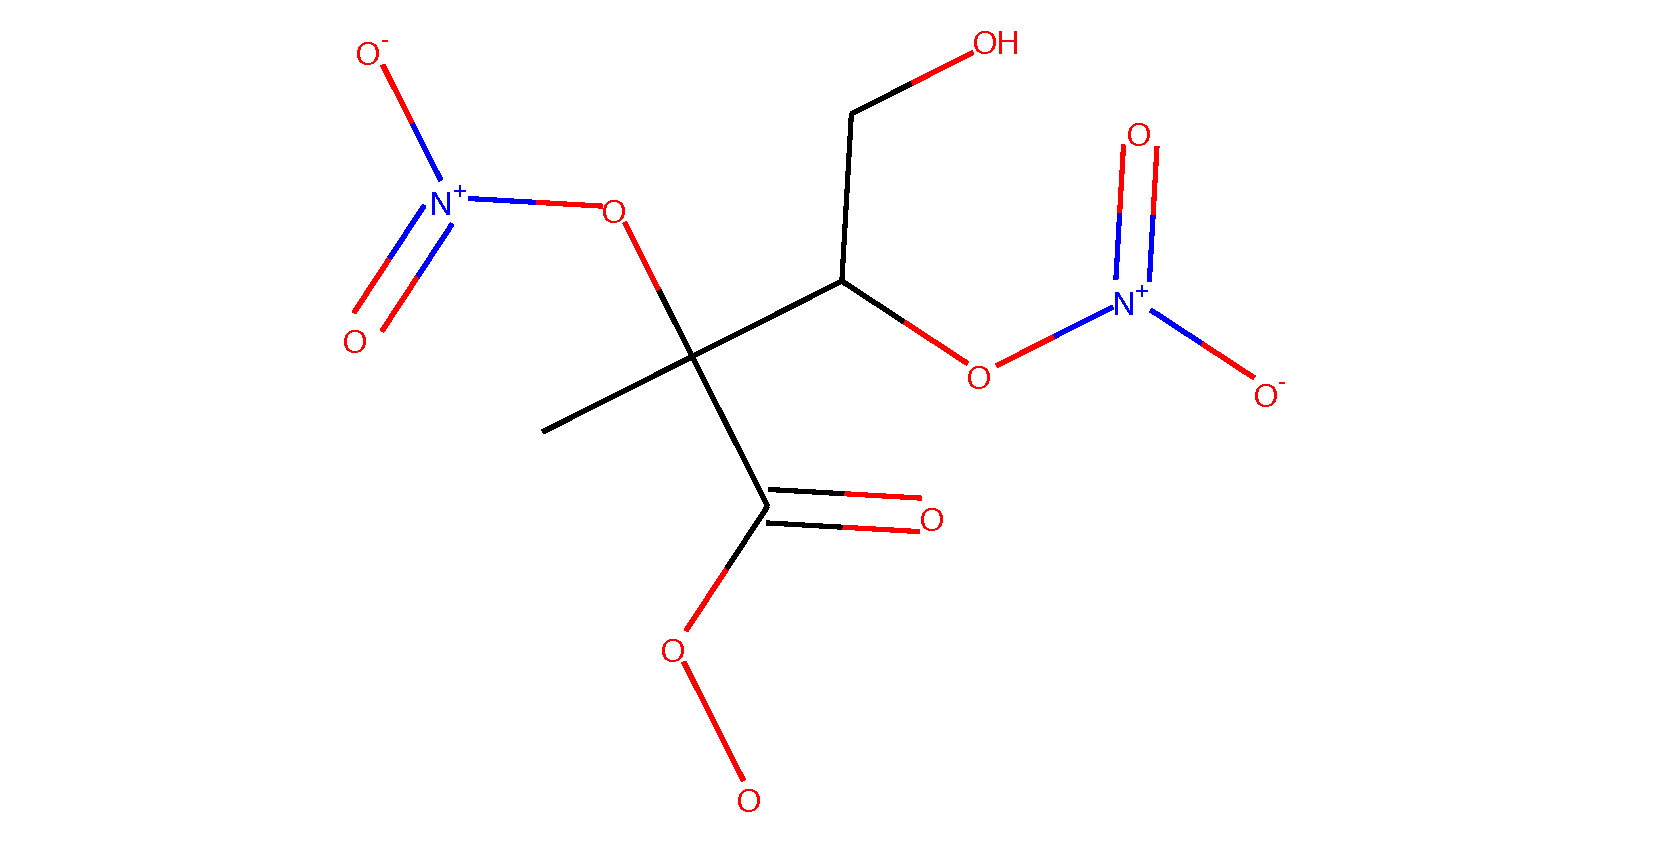
\includegraphics[width=\textwidth,height=.8\textwidth]{4fig/INB1NBCO3.pdf}
         \caption{Chemical structure drawn using \citep{rdkit}}
         \label{fig:graphmol}
     \end{subfigure}
     \hfill
     \begin{subfigure}[b]{0.495\textwidth}
         \centering
         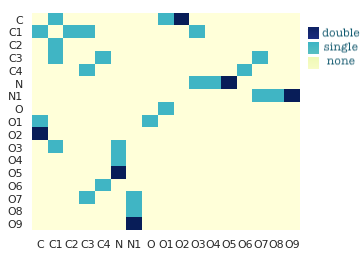
\includegraphics[width=\textwidth,height=.8\textwidth]{4fig/INB1NBCO3_adj.png}
         \caption{Corresponding adjacency matrix.}
         \label{fig:adjmol}
     \end{subfigure}

        \caption{ The molecular structure of \ce{INB1NBCO3}, one of the more functionalized species in the MCM, represented as a graph with nodes of consisting of either Oxygen, Carbon or Nitrogen and its adjacency matrix. Note that this is symmetrical since bonds are not directional.}
        \label{fig:bondmat}
\end{figure}


\paragraph{MCM graph: Node Embeddings}\label{sec:n2vec}

As shown in chapter YYY, representing the reactions within a mechanism in the form of a graph exposes patterns presented by the generation protocol, and thus the species chemical structure. We saw this through the categorisation of graph structures into aromatics, terpenes and an alkane/alkenes REF, and through van-krevelin ratios showing the progressive oxidation of species, to the production of \ch{Co2} (CO in the mcm) and water, \autoref{fig:vk}.


\begin{figure}[h]
  \centering
  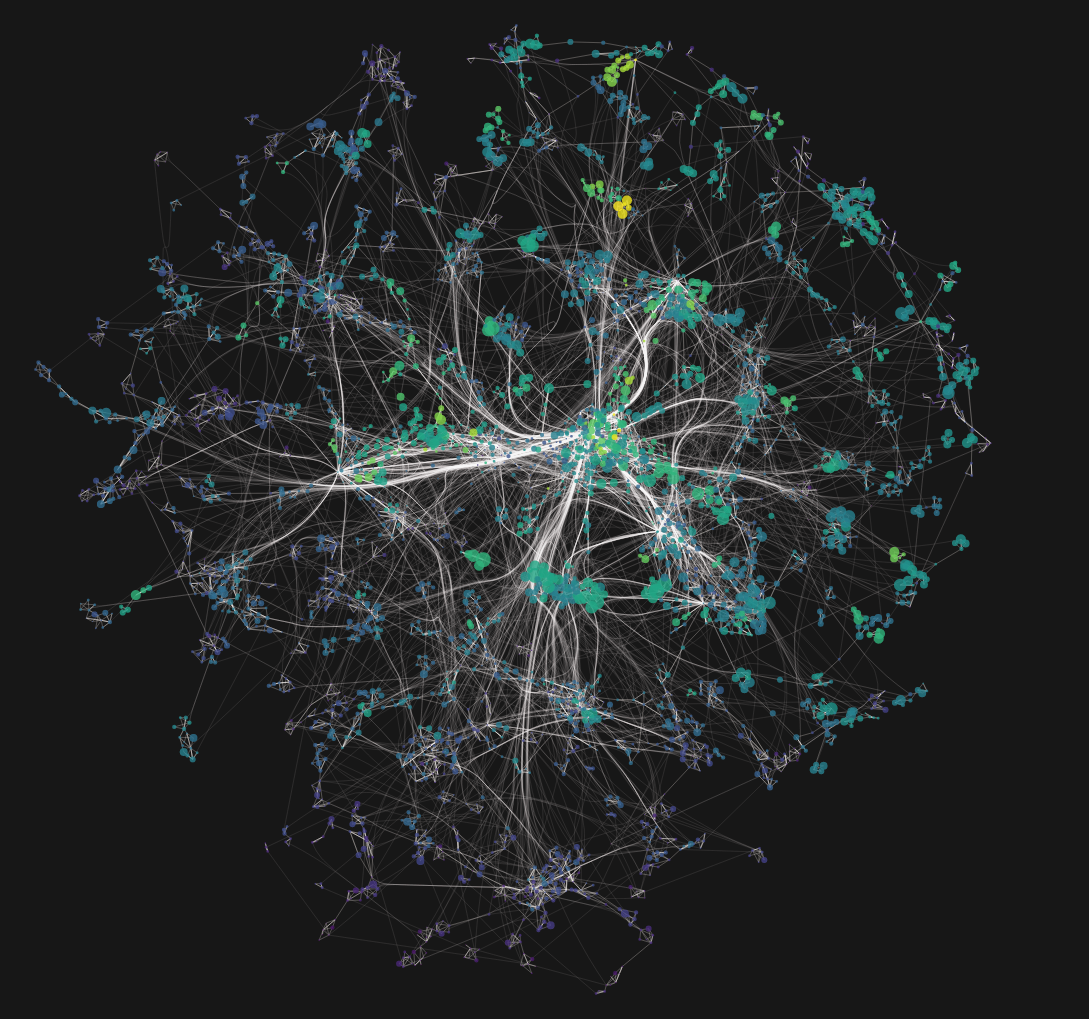
\includegraphics[width=\textwidth]{4fig/graph/oxidised_ratio.png}
  \caption{A graph representing the MCM mechanism derived from measured emissions in Beijing. This shows an increase of the O-C ratio as species are oxidised towards CO (center).  }
  \label{fig:vk}
\end{figure}


We can make use of the fact that chemical structure is encoded within the mechanism through its construction process. To extract this we may use node2vec, \citep{node2vec}, a program used to covert the structure of a graph into a numerical vector for use in machine learning. This is discussed in detail in  \autoref{sec:n2v}.




\subsubsection{Molecular Fingerprints}\label{sec:fingerprints}
Molecular fingerprints (structural keys) are a way of encoding molecule structure into a queryable series of binary digits. These are predominately used in the filed of chemical-informatics as means of exploring chemical space (a type of property space constructed using pre-determined properties and boundary conditions). Properties are often split into structural and psyico-chemical groups, allowing for the use of data mining techniques in search of molecule similarity (with uses such as the discovery of natural analogues to circumvent side effects and in-tolerances \citep{analog}). Unlike line notations, such as smiles and InChi, molecular fingerprints provide a multi-dimensional classification for chemical species which makes them ideal for machine learning inputs.

\paragraph{Molecular Quantum Numbers (MQN)}
In chemistry the shape, phase and electron occupancy of an atom may be described through the use of four quantum numbers\footnote{These are $n$ principle quantum number, $I$ angular momentum quantum number, $M_i$ magnetic quantum number and $M_s$ spin quantum number.}. The rationalisation of elements based on their structure, and by consequence reactivity, has led to the most iconic tool of the modern-day chemist - the periodic table\footnote{Increasing atomic numbers follow the principal quantum number.} \citep{periodic}. In representing a molecule as a set of 42 quantum numbers, MQN fingerprints produce a multi-dimensional mapping of atom, bond, polarity and topology count \citep{MQN}. Its binary nature not only... application..

[ref fae others... ]

\paragraph{Molecular ACCess System (MACCS)}
MACCS keys are a 164\footnote{Although they are 166-bit keys, there is no real agreement to what the 44th keys' purpose is, and therefore it is often omitted. Within RDKIT this is denoted by a $?$ \citep{rdkitcode}.} bit structural keys formulated through answering a series of structure-related questions. Developed by MDL Information Systems \citep{maccs}, their main purpose lies in being a SMILES Arbitrary Target Specification (SMARTS) system for substructure searching. However their distinct structure key format

makes them highly suitable for similarity detection. In many cases, the optimised version of MACCS keys is cited (\citep{optimised}), although most use cases exploit a variation of the undocumented 166bit keys. We use the implementation presented by \citep{rdkit,rdkitcode} for all molecular fingerprints in this section.
